\subsection{Important definitions}

\begin{definition}
    The standard simplex of dimension $n$ is the following subset of
    $R^{n+1}$, 
    $$\Delta_n = \{x = (x_1, ..., x_{n+1}) \in \R^{n+1} | \forall i, x_i \ge 0
    \text{ and } \sum_{i=1}^{n+1} x_1 = 1\}.$$

    For any collection of points $a_1, ..., a_k \in \R^n$, we define their
    convex hull as:
    $$  
    conv(\{a_1, ..., a_k\}) = \left\{\sum_{1\le i \le k} t_i a_i | \sum_{1 \le i \le k} t_i = 1, t_1, ..., t_k \ge 0\right\}
    $$
\end{definition}

\begin{definition}
    Let $V$ be a set (called the set of vertices). A simplicial complex over
    $V$ is a set $K$ of subsets of $V$ (called the simplices) such that, for
    every $\sigma \in K$ and every non-empty $\tau \subset \sigma$, we have
    $\tau \in K$. If $\sigma \in K$ is a simplex, its non-empty subsets $\tau
    \subset \sigma$ are called faces of $\sigma$, and $\sigma$ is called a
    coface of $\tau$. Moreover, its dimension is $|\sigma| - 1$ and the
    dimension of a simplicial is the maximum dimension of its simplices. 
\end{definition}

\begin{definition}
    Let $K$ be a simplicial complex, with vertex $V = [\![1,n]\!]$. In
    $\R^{n}$, consider, for every $i \in [\![1,n]\!]$, the vector $e_i = (0,
    ..., 1, 0, ..., 0)$ (i$^{th}$ coordinate $1$, the other ones $0$). Let
    $|K|$ be the subset of $\R^{n}$ defined as: 
    $$|K| = \bigcup_{\sigma \in K} conv(\{e_j , j \in \sigma\}).$$ Endowed with the subspace topology, $(|K| , T_{||K|}
)$ is a topological space, that we call the \textbf{topological realization} of $K$.
\end{definition}

\begin{definition}
    Let $(X, \T)$ be a topological space. A triangulation of $X$ is a
    simplicial complex $K$ such that its topological realization $(|K| , T_{||K|})$ is homeomorphic to $(X, \T)$.
\end{definition}

\begin{definition}
    Let $K$ be a simplicial complex of dimension $n$. Its Euler characteristic
    is the integer
    $$\chi(K) = \sum_{0 \le i \le n} (-1)^i \cdot \text{(number of simplices
    of dimension i)}.$$
\end{definition}

\begin{definition}
    The Euler characteristic of a topological space is the Euler
    characteristic of any triangulation of it.
\end{definition}

\subsection{Exercises}

\begin{exercise}
    Give a triangulation of the cylinder.
\end{exercise}

\begin{proof}

We can think a triangulation of the cylinder in that following form: each circular section is mapped
into a triangle graph. On the other hand, the line can be mapped to an edge.
Since a cylinder can be written as $\sphere_1 \times \R$, the triangulation
as well. 

Let's write
down: 
$$K = \{[0,1,3], [0,2,3], [2,3,5], [2,4,5],[4.5,1],[4,1,0]\}$$

\begin{figure}[H]
    \begin{center}
        \tikzset{every picture/.style={line width=0.75pt}} %set default line width to 0.75pt        

        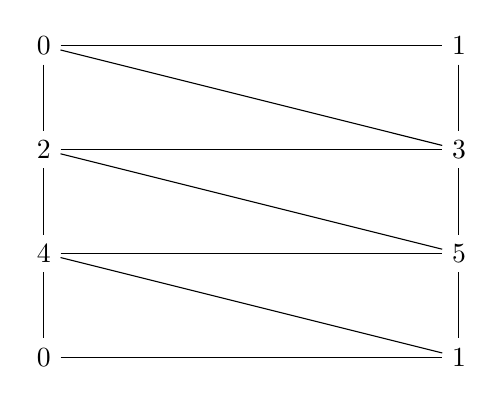
\begin{tikzpicture}[x=0.75pt,y=0.75pt,yscale=-1,xscale=1]

        \node (zero) at (0,0){0};
        \node (one) at (200,0){1};
        \node (two) at (0,50){2};
        \node (three) at (200,50){3};
        \node (four) at (0,100){4};
        \node (five) at (200,100){5};
        \node (zero1) at (0,150){0};
        \node (one1) at (200,150){1};

        \draw (zero) -- (one);
        \draw (two) -- (three);
        \draw (four) -- (five);
        \draw (zero1) -- (one1);
        
        \draw (zero) -- (two) -- (four) -- (zero1);
        \draw (one) -- (three) -- (five) -- (one1);
        
        \draw (zero) -- (three);      
        \draw (two) -- (five); 
        \draw (four) -- (one1);

        \end{tikzpicture}
    \end{center}
\end{figure}

\end{proof}

\noindent\linia

\begin{exercise}
    What are the Euler characteristics of Examples 4.5 and 4.6? What is the Euler characteristic of the icosahedron?
\end{exercise}

\begin{proof}

\textbf{Exemplo 4.5:} 
$$K = \{[0], [1], [2], [3], [0, 1], [1, 2], [2, 3], [3, 0], [0, 2], [1, 3], [0, 1, 2], [0, 1, 3], [0, 2, 3], [1, 2, 3]\}.$$
$$
\chi (K) = 4 - 6 + 4 = 2
$$

\textbf{Exemplo 4.6:}
\begin{multline*}
    K = \{[0], [1],[2], [3], [0, 1], [1, 2], [1,3], [0,2] ,[2, 3], [3, 0], \\
    [0, 1, 2], [0, 1, 3], [0, 2, 3], [1, 2, 3], [0, 1, 2, 3]\}.    
\end{multline*}
$$
\chi (K) = 4 - 6 + 4 - 1 = 1
$$

\textbf{D20:} It has 20 faces (dimension 2), 30 edges (dimension 1) and 12
vertices (dimension 0), its Euler characteristic is $12 - 30 + 20 = 2$ (Euler
relation).

\end{proof}

\noindent\linia

\begin{exercise}
    Let $K$ be a simplicial complex (with vertex set $V$). A sub-complex of
    $K$ is a set $M \subset K$ that is a simplicial complex. Suppose that
    there exists two sub-complexes $M$ and $N$ of $K$ such that $K = M \cup
    N$. Show the inclusion-exclusion principle:
    $$
    \chi(K) = \chi(M) + \chi(N) - \chi(M \cap N)
    $$
\end{exercise}

\begin{proof}

Denote $k_i$ the number of simplices of dimension $i$, that is, $\chi (K) =
\sum_{0 \le i \le k} (-1)^i k_i$, with $k$ being its dimension. Each simplex of dimension $i$ belongs to
$M$, to $N$ or both. Denote $k_i^M, k_i^N$ and $k_i^{MN}$ the number od
simplices of dimension $i$ in $M$, $N$ and $M \cap N$ respectively. So
$$k_i = k_i^M + k_i^N - k_i^{MN}.$$
Therefore, 
$$
\chi(K) = \sum_{0 \le i \le k} (-1)^i (k_i^M + k_i^N - k_i^{MN}) = \sum_{0 \le i \le k}(-1)^i k_i^M + \sum_{0 \le i \le k}(-1)^i k_i^N - \sum_{0 \le i \le k}(-1)^i k_i^{MN} 
$$
Let $m$ and $n$ be the dimension of $M$ and $N$,
respectively. Now I shall prove $M \cap N$ is a simplicial complex. Take
$\sigma \subset M \cap N$ and $\tau \subset \sigma$, then $\tau \subset \sigma
\in M$ and $\tau \subset \sigma \in N$, what implies $\tau \in M \cap N$. It
proves its a simplicial complex with dimension $p$. We know the dimension of $M$ is
$m$, so it implies that for all $i > m$, $k_i^M = 0$. Suppose not and let $k_j^M > 0$ for
some $j > m$, we would have a simplex with dimension greater or equal than
$m$. This is a contradiction, because the the dimension of $M$ is the maximum
dimension of its simplices. This holds for $N$ and $M \cap N$. 
$$
\chi(K) = \sum_{0 \le i \le k} (-1)^i (k_i^M + k_i^N - k_i^{MN}) = \sum_{0 \le i \le k}(-1)^i k_i^M + \sum_{0 \le i \le k}(-1)^i k_i^N - \sum_{0 \le i \le k}(-1)^i k_i^{MN} 
$$
We conclude that 
$$
\chi(K) = \sum_{0 \le i \le m}(-1)^i k_i^M + \sum_{0 \le i \le n}(-1)^i k_i^N - \sum_{0 \le i \le p}(-1)^i k_i^{MN} = \chi(M) + \chi(N) - \chi(M \cap N)
$$
    
\end{proof}

\noindent\linia

\begin{exercise}
    What is the Euler characteristic of a sphere of dimension 1? 2? 3? 
\end{exercise}

\begin{proof}

We may find the Euler characteristic of one triangulation of the sphere. So we
first need to find a triangulation for the sphere $\sphere_n \subset
\R^{n+1}$. We can think in the simplex in this space. In $\R^2$ it's the
triangle, in  $\R^3$ it's the tetrahedron, in $\R^4$ it's the 5-cell and so
on. The simplex in $\R^{n+1}$ has $n + 2$ vertices and each vertex connect to
all the other. We have also $n+2$ simplices of dimension $n$, because each
has $n+1$ points, that is, $\genfrac(){0pt}{}{n+2}{n+1} = n+2$. For each of them, we
must include all its subsets. 

Now we can calculate the Euler characteristic for each triangulation and
therefore each sphere. 

$$
\chi(\sphere_1) = -3 + 3 = 0 
$$
$$
\chi(\sphere_2) = 4 - 6 + 4 = 2 
$$
$$
\chi(\sphere_3) = -5 + 10 - 10 + 5 = 0  
$$
$$
\chi(\sphere_4) = 6 - 15 + 20 - 15 + 6 = 2  
$$

    
\end{proof}

\noindent\linia

\begin{exercise}
    Using the previous exercise, show that $\R^3 - \{0\}$ and $\R^4 - \{0\}$ are not homotopy equivalent.
\end{exercise}

\begin{proof}

Suppose that $\R^3 - \{0\}$ and $\R^4 - \{0\}$ are homotopy equivalent. By
Example 3.15, $\sphere_{n-1}$ is homotopic equivalent to $\R^n - \{0\}$. By
this and using the transitive property we conclude that $\sphere_2$ and
$\sphere_3$ are homotopic equivalent. If that is true, we infer that they have
the same Euler characteristic, what is a contraction by the last exercise.
Hence $\R^3 - \{0\}$ and $\R^4 - \{0\}$ are not homotopy equivalent.

\end{proof}

\noindent\linia

The computational exercises (22 - 26) can be found in the
Github\footnote{\url{github.com/lucasmoschen/topological-data-analysis/blob/main/tutorials/tutorial-1.ipynb}}

\begin{exercise}
    Build triangulations of the letters of the alphabet, and compute their Euler characteristic.
\end{exercise}

\begin{exercise}
    For every $n$, triangulate the bouquet of $n$ circles (see below). Compute
    their Euler characteristic.
\end{exercise}

\begin{exercise}
    Implement the following triangulation of the torus.
\end{exercise}

\begin{exercise}
    Consider the following dataset of 30 points $x_0, ..., x_{29}$ in $R^2$.

    Write a function that takes as an input a parameter $r \ge 0$, and returns
    the simplicial complex $\mathcal{G}(r)$ defined as follows:
    \begin{enumerate}
        \item the vertices of $\mathcal{G}(r)$ are the points $x_0, ..., x_{29}$,
        \item for all $i, j \in [[0, 29]]$ with $i \neq j$, the edge $[i, j]$ belongs to $\mathcal{G}(r)$ if and only if
        $||x_i - x_j|| \le r$.
    \end{enumerate}
    
    Compute the number of connected components of $\mathcal{G}(r)$ for several
    values of $r$. What do you observe?
\end{exercise}

\begin{exercise}
    A Erdos–Renyi random graph $\mathcal{G}(n, p)$ is a simplicial complex
    obtained as follows:
    \begin{enumerate}
        \item add $n$ vertices $1, ..., n$,
        \item for every $a, b \in [[1, n]]$, add the edge $[a, b]$ to the complex with probability $p$.
    \end{enumerate}

    Builds a function that, given $n$ and $p$, outputs a simplicial complex $\mathcal{G}(n, p)$. Observe
    the influence of $p$ on the number of connected components of $\mathcal{G}(10, p)$ and $\mathcal{G}(100, p)$.
\end{exercise}